\chapter{Tracker Data Quality Monitoring}
\label{chap:trackdqm}

The current methods for data certification require a large amount of person-power. For instance, for Offline Tracker DQM, shifters undertake eight-hour shifts in which they look at hundreds of monitoring histograms which describe what happened during each run under evaluation. Two issues arise with this approach. Firstly, the increasing data volume and detector complexity, especially when the age of the High-Luminosity LHC (HL-LHC) arrives, means that shifters will have to look at more aspects of the detector in order to make decisions of the data quality, slowing down the data certification process and leading to higher mental strain, a possible source of human error. Moreover, the amount of monitoring histograms each shifter will have to look at in order to make a fair assessment will increase drastically, an issue which compounds the already existing problem of a lack of per-LS certification due to monitoring histograms being integrated over the entire run. The latter issue of low certification granularity may result in the certification of anomalous LSs as good, leading to the inclusion of problematic data downstream in the physics analyses performed by the collaboration.

The aforementioned issues require a new approach. Thus, the CMS Collaboration has taken on the task of developing tools that aim to automate the detector monitoring and data certification process with higher granularity (i.e. per-LS) \cite{wachirapusitanMachineLearningApplications2023, brinkerhoffAnomalyDetectionAutomated2025, CMS-DP-2021-034}. One of the main approaches towards tackling this problem has been through the integration of anomaly detection machine learning (ML) techniques in order to flag anomalous per-LS monitoring histograms, which a shifter can then manually evaluate. Unfortunately, until recently, there has been no accessible way for shifters to evaluate runs per LS.

\section{DQM Explore}

To address the limited access to per-LS information and to have a standard system to apply ML models for anomaly detection for DQM data, the Data Inspector for Anomaly Detection (DIALS) Web app was developed as a central tool for data visualization and ML training and inference \cite{CmsdqmdcServicesDialsservice2025}. Although DIALS offers an Python API through which one can obtain per-LS monitoring histogram data, there is currently no programmatic way to explore or visualize these data. Additionally, while the web app allows the user to these monitoring histograms per-LS, the UI is not optimized for the type of dynamic and interactive data exploration that would allow a shifter or expert to track the evolution of anomalies through time. This limitation led to the initial development of DQM Explore.

DQM Explore is a Python toolkit which offers utilities for programmatic access and exploration of DQM data, including per-LS monitoring histograms through the DIALS API, information on data-taking conditions through the CMS Online Monitoring System (OMS) API, and Offline Tracker Certification information such as used reference runs from the Certification Helper (CH) web app. It's flagship feature is the ability to construct interactive per-LS monitoring histograms that allow for easy tracking of the evolution of runs. Work is currently underway to incorporate these tools into DIALS in order to enhance the webapp's data exploration capabilities and facilitate the analysis of anomalous LSs by shifters, shift leaders and experts. However, despite this work still being pending, these tools have already served to facilitate the investigation of anomalous LSs by experts. In the following section, we discuss an erroneous certification that was fixed due to the heightened granularity provided by the per-LS plots made with DQM Explore which allowed experts to investigate the anomalous LSs.

\subsection{Case Study: Run 380238}

Run 380238 is a proton-proton collision run which was done in era C of data taking in 2024. A notable feature of this run was that during the first 10 LSs, a certain number of front-end drivers (FEDs) in the Pixel detector showed zero hits, as seen in Figure \ref{fig:digi_fed_380238}, pointing to a potential time-localized anomaly. This issue was reflected in a localized lower number of digitizations in the two-dimensional histogram for each of the four Pixel detector layers, as can be seen in Figure \ref{fig:digimaps_380238}. However, although the issue was noted, because the track quality seemed unaffected as illustrated in Figure \ref{fig:380238trkqual}, and because the ability to evaluate these time-localized issues was limited, the run was certified as good by the offline tracker shifter which evaluated it.

\begin{figure}[h]
    \centering
    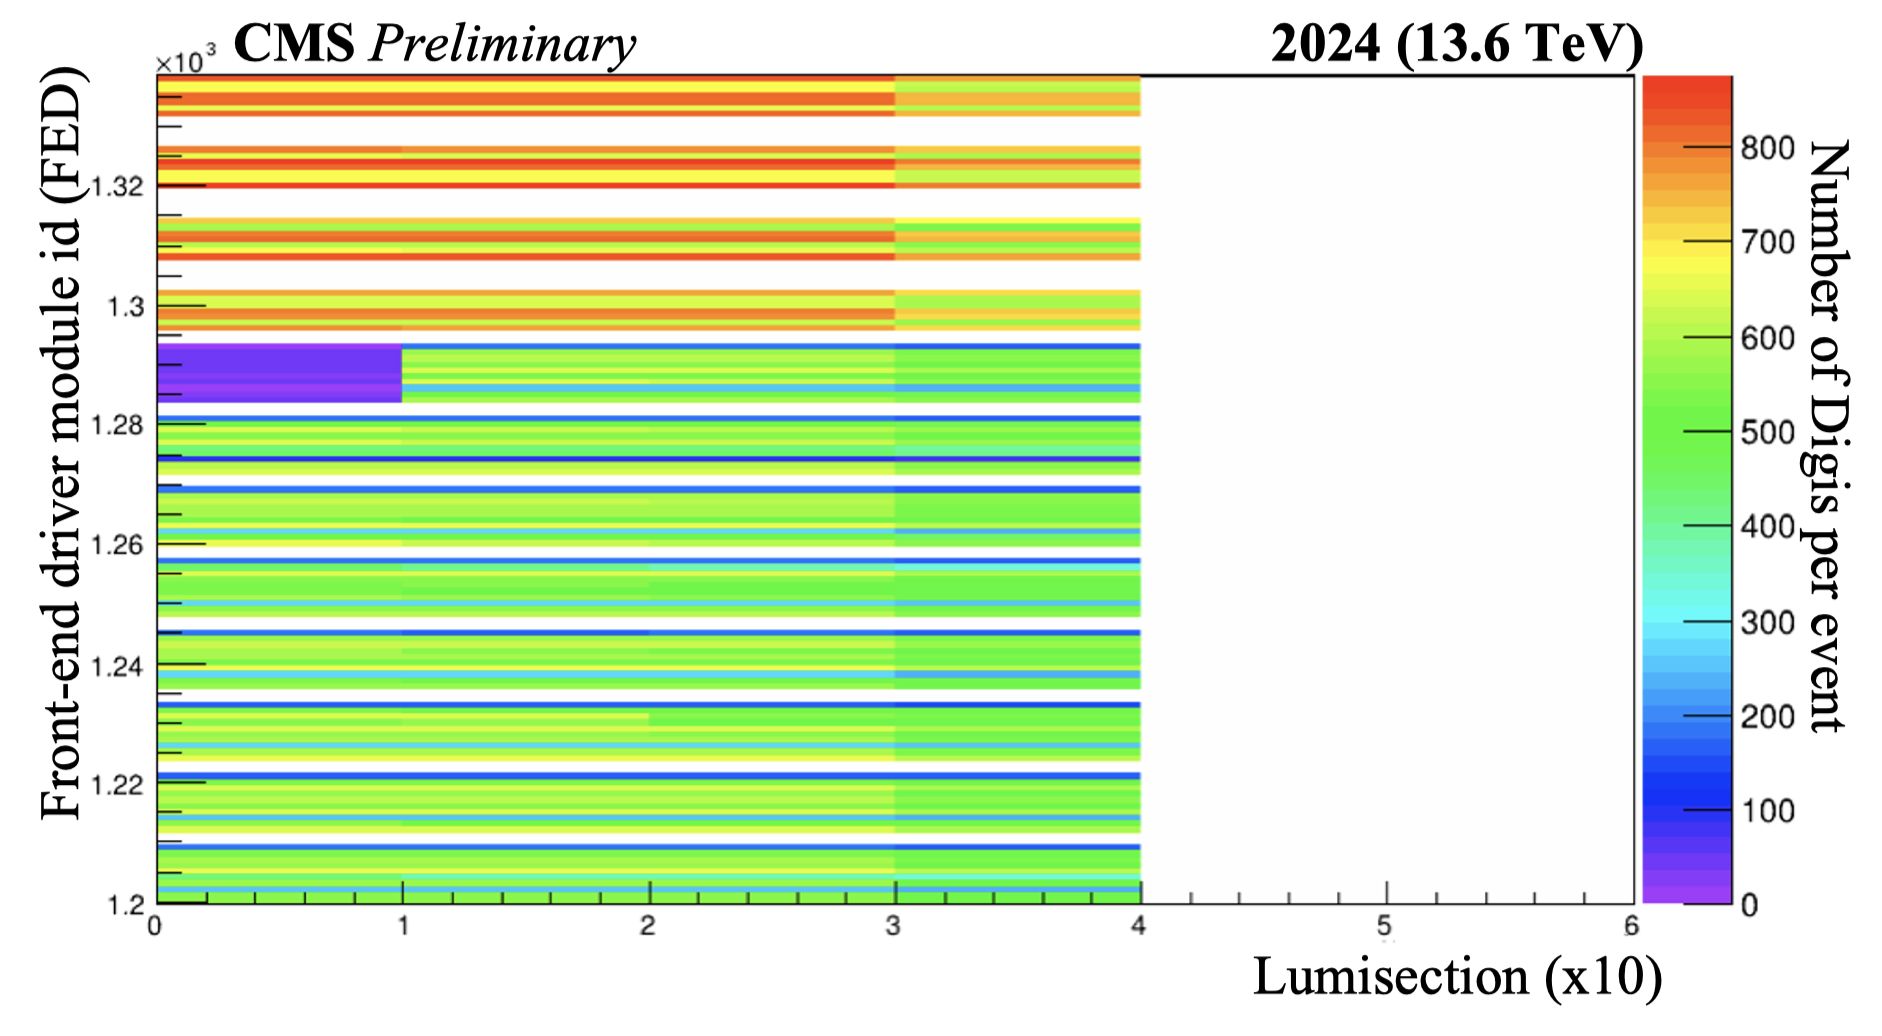
\includegraphics[width=0.5\linewidth]{images/digi_fed_380238.png}
    \caption{Plot of the time evolution of the total number of digitizations for each FED in the Pixel detector \cite{CMS-DP-2024-070}. The first 10 LSs show anomalous behavior of a subset of FEDs.}
    \label{fig:digi_fed_380238}
\end{figure}

\begin{figure}[h]
  \centering
  \begin{tabular}{cc}
    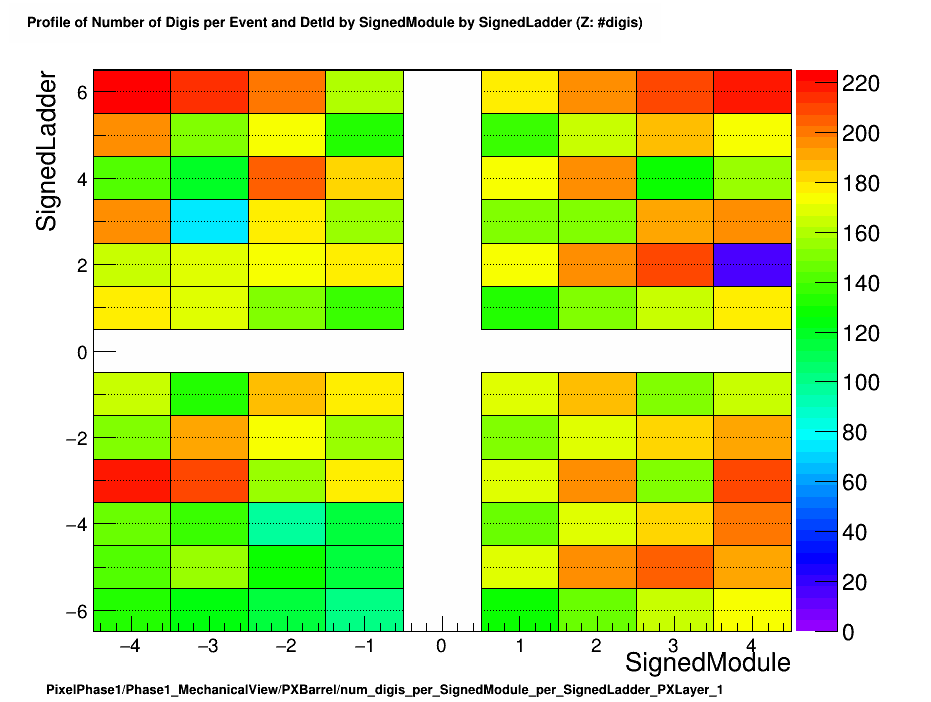
\includegraphics[width=0.4\textwidth]{images/num_digis_per_SignedModule_per_SignedLadder_PXLayer_1.png} & 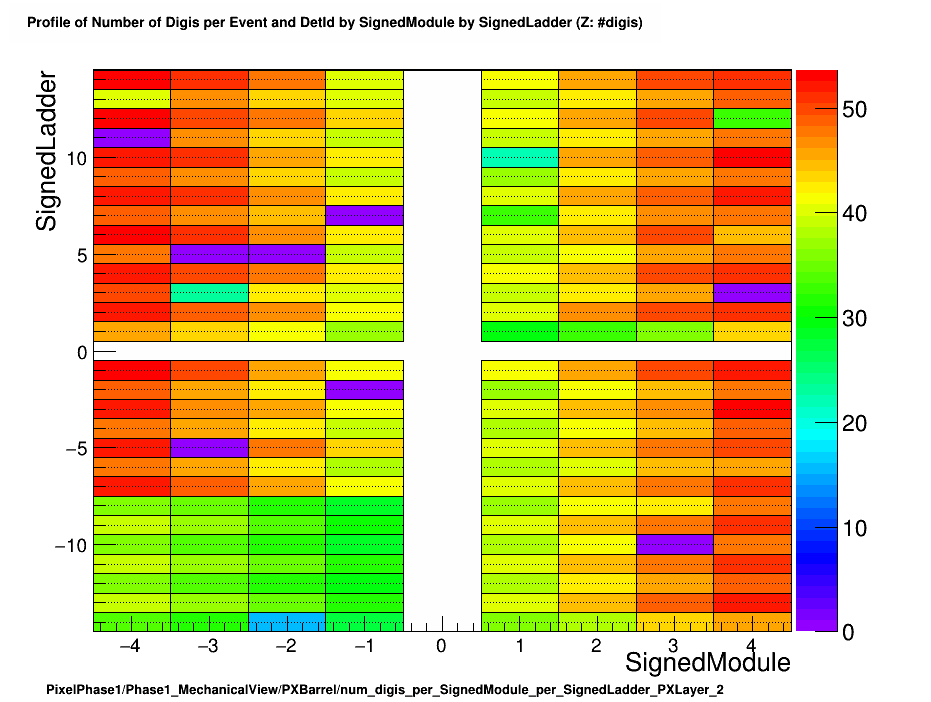
\includegraphics[width=0.4\textwidth]{images/num_digis_per_SignedModule_per_SignedLadder_PXLayer_2.png} \\
    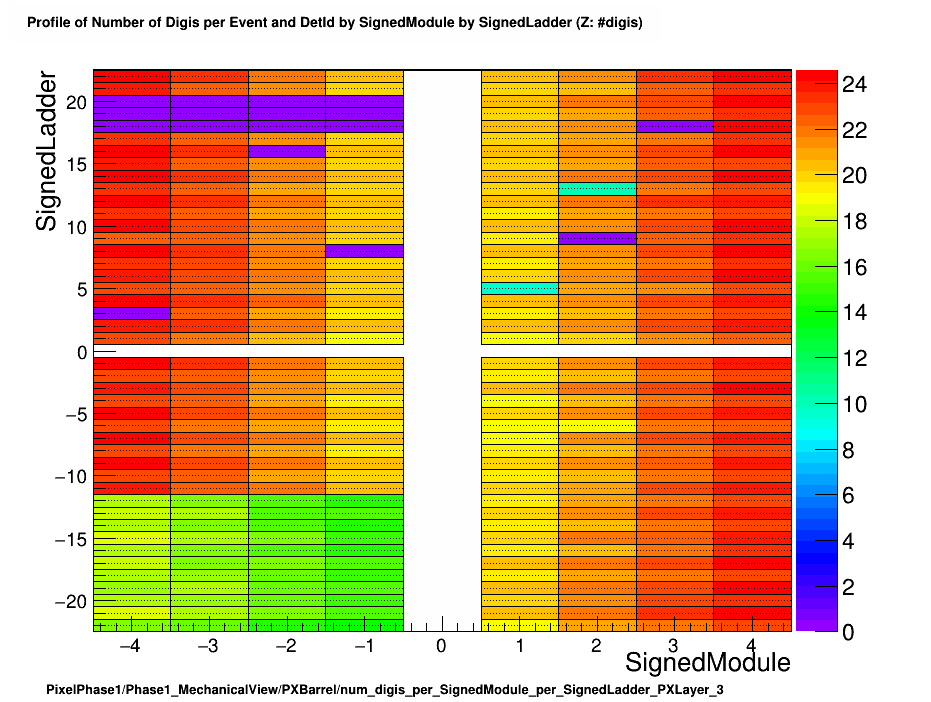
\includegraphics[width=0.4\textwidth]{images/num_digis_per_SignedModule_per_SignedLadder_PXLayer_3.png} & 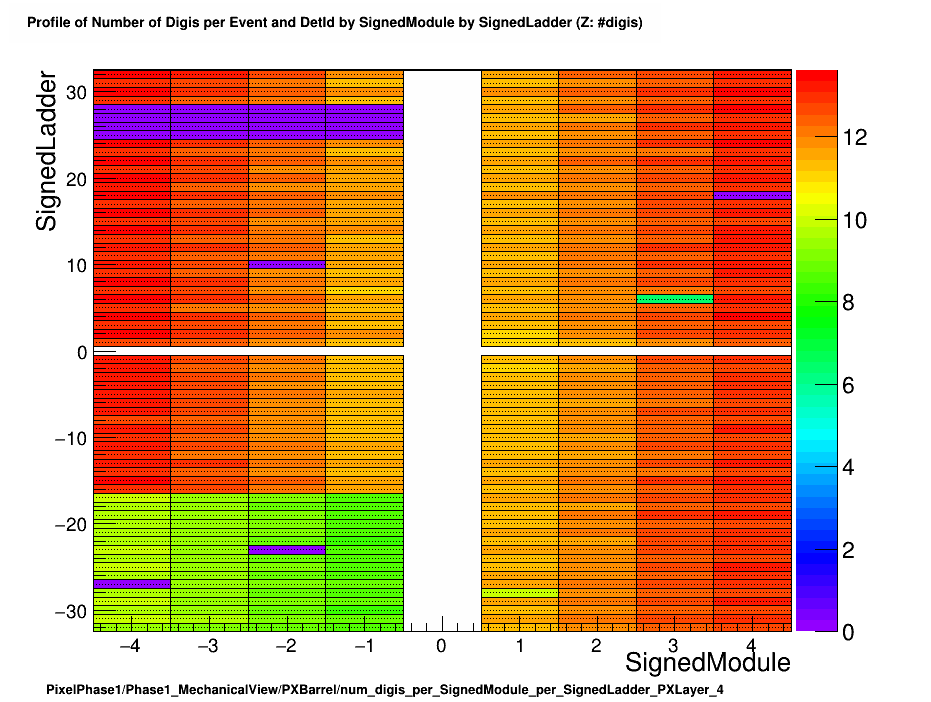
\includegraphics[width=0.4\textwidth]{images/num_digis_per_SignedModule_per_SignedLadder_PXLayer_4.png} \\
  \end{tabular}
  \caption{Digitization maps for all layers of the Pixel detector in 380238.}
  \label{fig:digimaps_380238}
\end{figure}

\begin{figure}[h]
  \centering
  \begin{minipage}{0.45\textwidth}
    \centering
    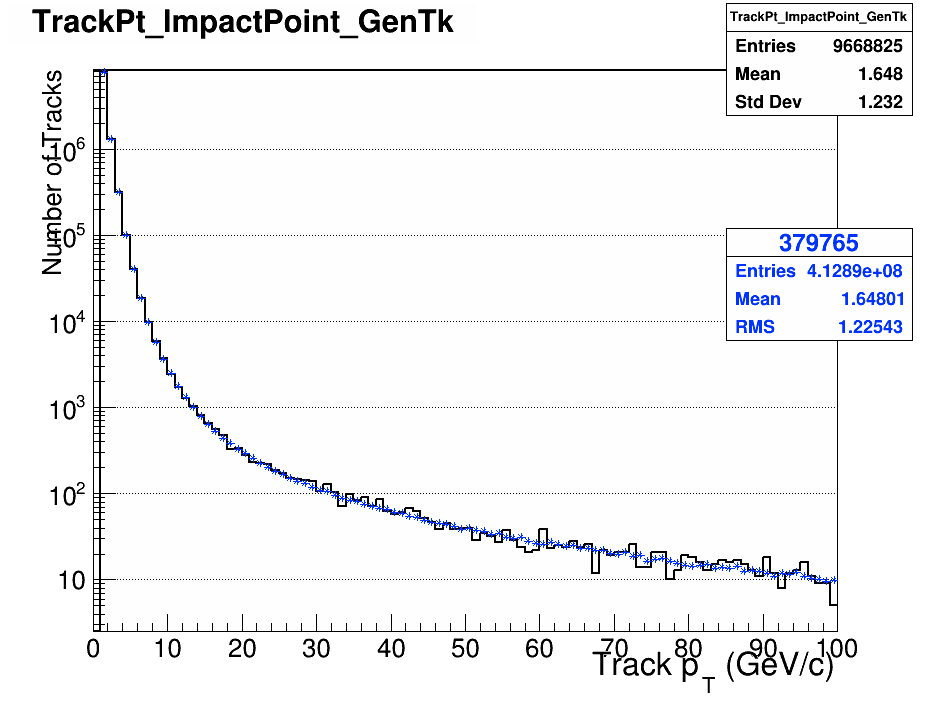
\includegraphics[width=\textwidth]{images/trackpt380238.png}
  \end{minipage}
  \hfill
  \begin{minipage}{0.45\textwidth}
    \centering
    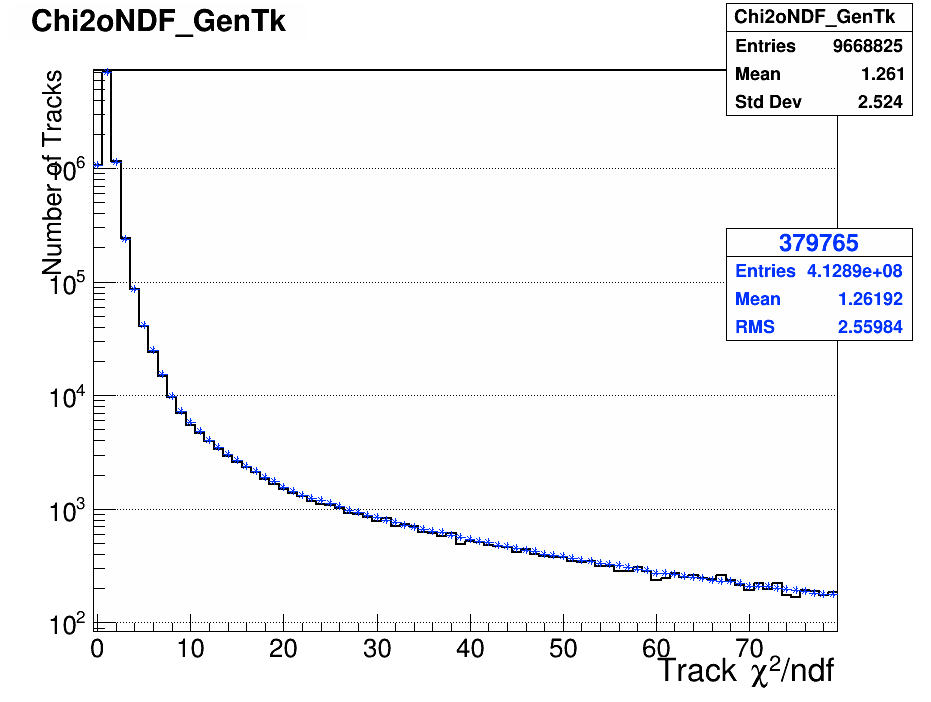
\includegraphics[width=\textwidth]{images/chi2ondf380238.png}
  \end{minipage}
  \caption{Example monitoring elements for run 380238 reflecting the nominal nature of the track quality of this run when compared to the reference run 379765. On the left is the $p_T$ histogram of the reconstructed tracks and on the right is the $\frac{\chi^2}{\text{NDF}}$ histogram for the fit of these tracks to the hits detected by the Pixel.} 
  \label{fig:380238trkqual}
\end{figure}

Some time after this initial certification, experts used the DQM Explore per-LS interactive plotting tools to scrutinize this run more closely. The interactive plots produced allowed experts to better understand the severity of the observed anomaly. Figure \ref{fig:380238lss} shows the resulting plots from this evaluation, which show that the regions in each layer that had low digitization in the integrated summary digitization histogram which the DQMGUI offered was due to there being no digitizations at all during the first 10 LSs, meaning that about $1/8$ of each Pixel layer was off, exceeding the expected severity for this issue. With these results, the certification for this run was modified to reflect the reality: the first 10 LSs were certified as bad, while the rest, where the issue disappears, were certified as good. Upon further investigation, experts determined that the issue was caused by a low voltage trip \cite{CMS-DP-2024-070}. 

\begin{figure}[H]
  \centering
  \begin{minipage}{0.48\textwidth}
    \centering
    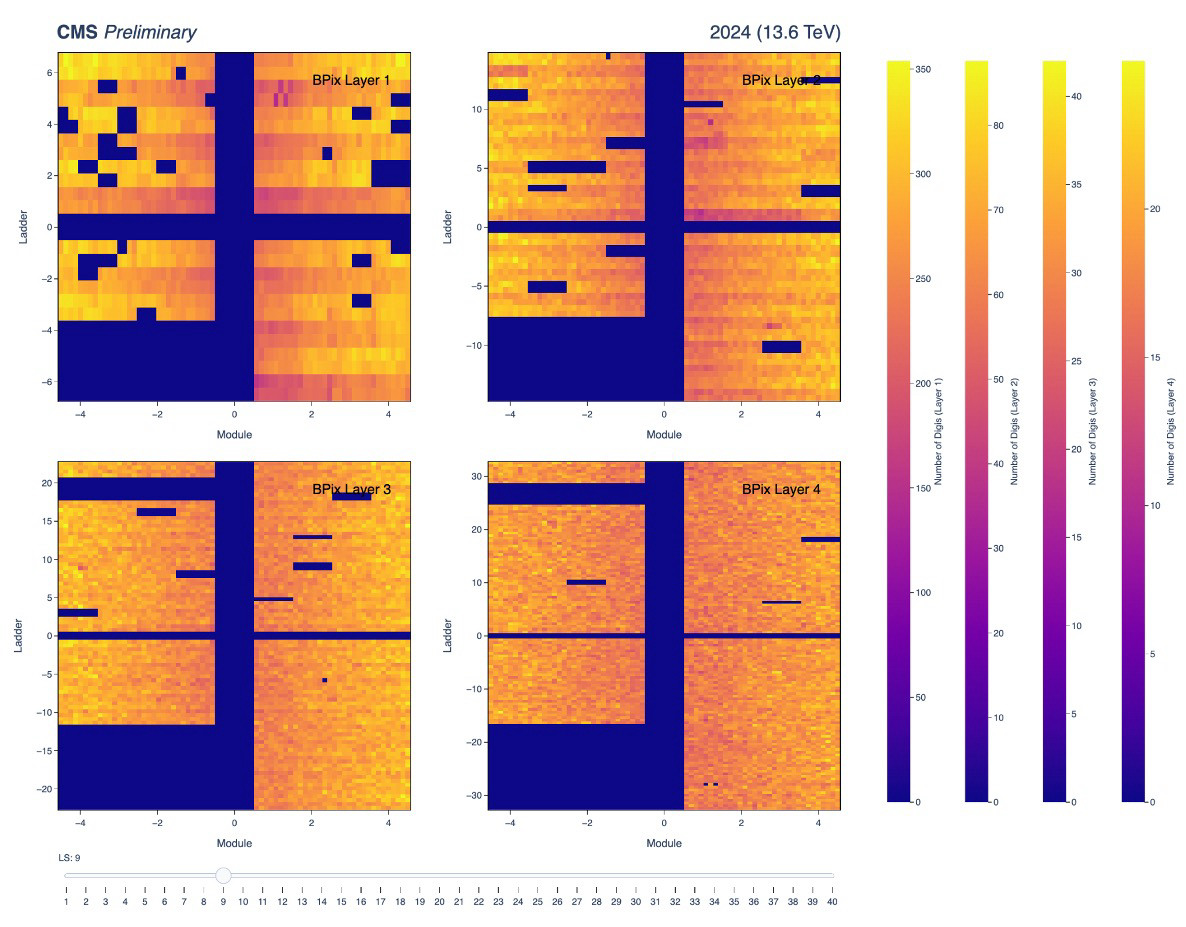
\includegraphics[width=\linewidth]{images/ls9.png}
  \end{minipage}
  \hfill
  \begin{minipage}{0.48\textwidth}
    \centering
    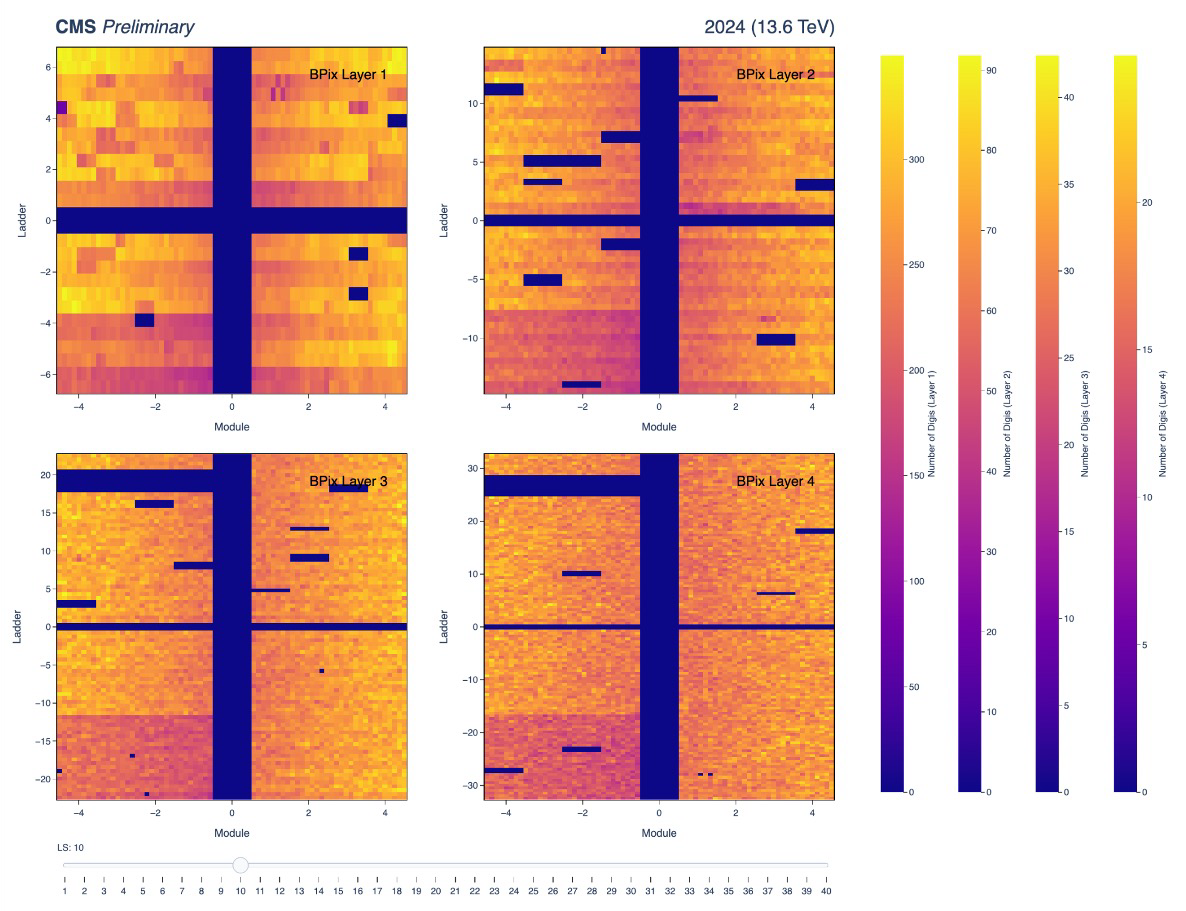
\includegraphics[width=\linewidth]{images/ls10.png}
  \end{minipage}
  \vfill
  \begin{minipage}{0.48\textwidth}
    \centering
    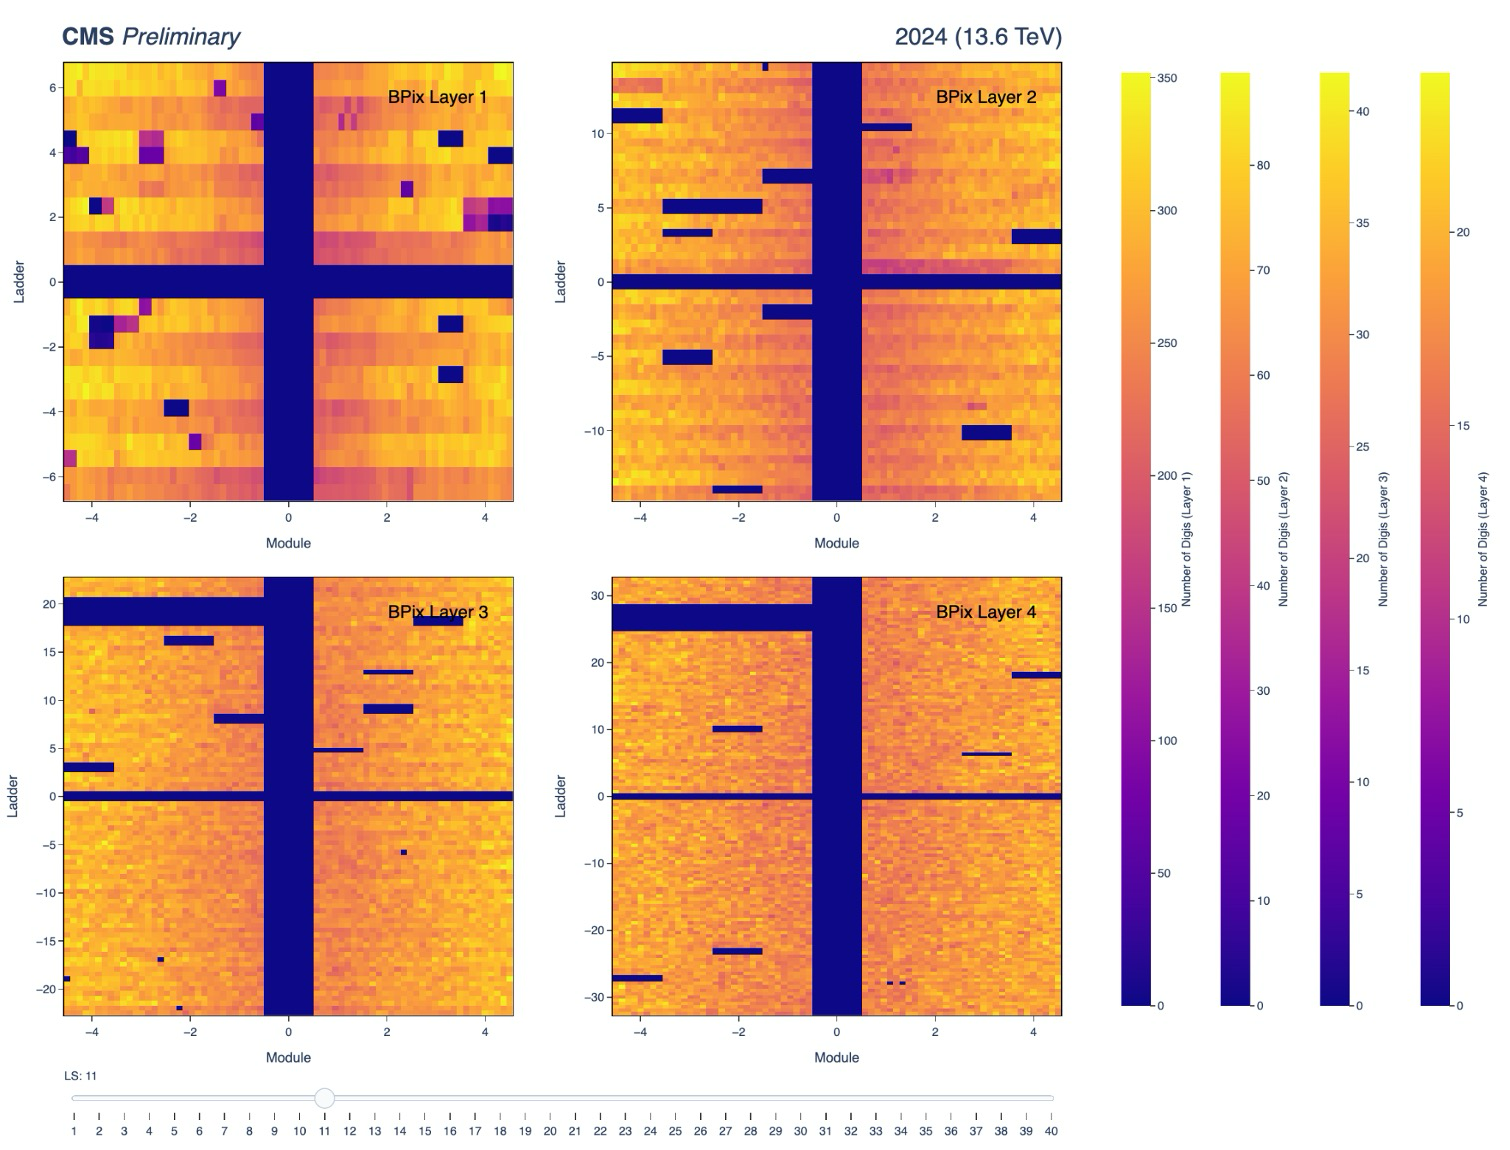
\includegraphics[width=\linewidth]{images/ls11.png}
  \end{minipage}
  \caption{Per-LS interactive plots of LSs 9 to 11 of run 380238, showing how the zero occupancy region recovered as the run progressed. These plots show all of the layers (layer 1 on the top left, 2 on the top right, 3 on the bottom left, and 4 on the bottom right).}
  \label{fig:380238lss}
\end{figure}

\section{Reference Run Ranking}

A challenge that arises when integrating ML into the data certification workflow is the question of what data to train the model on. During regular human-driven certification, reference runs (i.e. good, long runs with a lot of statistics) are used to compare runs with similar data-taking conditions that are being certified. Because these runs are carefully scrutinized by experts and have many LSs, they can serve as good training datasets for the ML models that are being implemented in DQM. 

One of the tools being developed which aim to facilitate the integration of ML into the certification process is the Reference Run Ranking (RRR) tool. This utility uses principal component analysis (PCA) and regularization to rank runs according to their similarity to the target run for which one wishes to find a reference run. The tool utilizes the API for the CMS Online Monitoring System (OMS), a webapp which provides comprehensive information on the detector status and data-taking conditions, in order to fetch per-run and per-LS features such as the magnetic field strength or the HLT physics rate which describe the conditions under which the data for any run was taken.

The RRR algorithm makes use of multiple data exploration tools provided by \texttt{DQMExplore}, such as an OMS data class which takes care of the retrieval and processing of data from OMS. It begins by first using the following inputs to fetch and format the data from OMS:

\begin{itemize}
    \item The number of the target run one wishes to find a reference run for.
    \item A selection and/or range of runs that will be considered candidate runs by the algorithm.
    \item Pre-filters on OMS features.
\end{itemize}

\noindent These inputs dictate the runs that will be fetched from the OMS API. The last of these, the prefilters, allow for the disqualification of runs which do not meet certain basic criteria. For example, we would not consider candidate runs with no magnetic field when the target run was taken with a magnetic field of $3.8 \text{ T}$, so it would be a waste of computational resources to fetch those data from OMS.

With the data fetched, the RRR then takes as input the specific data taking describing the features that will be used for the ranking. These features are divided into two categories: regular features and PCA features. For the former, the only transformation that is applied is regularization, which is done in order to remediate the potentially large difference in scale between each feature's range of values (e.g., magnetic field is $\mathcal O(1)\text{ Tesla}$, while the run number is $\mathcal O(10^5)$). This first set of features is given precedence during the ranking step, since they are utilized in their original form. In contrast, PCA features undergo dimensionality reduction via PCA, producing a set of principal components where the user can choose the number to employ.

With the features selected and processed, we then consider each run as being located in a high-dimensional abstract space where each axis corresponds to the constructed features. For instance, if we were to choose only \texttt{run\_number} and \texttt{b\_field} as the primary features, and the first principal component of a set of some PCA features, then this space would look like what is shown in Figure \ref{fig:RRRspace}\footnote{As is readily apparent from this figure, the algorithm makes the implicit assumption that all of the features in this abstract space are orthogonal. However, this is not necessarily the case, as there are certain features that can be highly correlated, such as the HLT trigger rate and luminosity.}.

\begin{figure}
    \centering
    \begin{tikzpicture}[>=Latex, line width=1pt]
      % Axes
      \draw[->] (0,0) -- (3,0) node[right] {PC1};
      \draw[->] (0,0) -- (0,3) node[right] {\texttt{run\_number}};
      \draw[->] (0,0) -- (-1.5,-1.5) node[below left] {\texttt{b\_field}};
    
      % Optional: origin dot
      % \filldraw[black] (0,0) circle (1pt);
    \end{tikzpicture}
    \caption{Schematic illustration of an example abstract space constructed for ranking by the RRR algorithm.}
    \label{fig:RRRspace}
\end{figure}

With the runs now in this abstract space, the algorithm then computes the Euclidean distance between the target run and the $i$-th candidate run using Equation \ref{eq:EclDist}, where $x$ corresponds to a primary feature, of which there are $N$ and $\text{PC}$ to a principal component, of which there are $P$.

\begin{equation}
    d_i = \sqrt{\sum_{n=1}^{N} (x_{\text{target},n} - x_{i,n})^2 +\sum_{p=1}^P (\text{PC}_{\text{target},p} + \text{PC}_{i,p})^2}
    \label{eq:EclDist}
\end{equation}

\noindent All candidate runs are then sorted in increasing order of distance. The candidate run at the top position is then considered the most similar (and thus the best potential candidate) for the target run for which we wish to find a reference run, the run in the second position the second most similar, etc. 

The development of RRR required and motivated the construction of a software infrastructure to obtain data from multiple sources, including OMS, Certification Helper, and, in part, DIALS. These tools were developed as part of the DQM Explore toolkit. Thus, a primary dependency of this algorithm is DQM Explore. Motivated by efforts to incorporate DQM Explore tools into DIALS, there are plans to add an automated ML training dataset and reference run selection tool which will be built based on RRR. However, before that is to materialize, work is being conducted in order to validate, test, and fine-tune the algorithm. The subsequent subsection will discuss some of these preliminary tests.

\subsection{Preliminary Studies}

A crucial test of RRR's ability to properly rank runs according to how well they would be as reference runs is whether or not it can replicate the decisions made by human experts. To test this, the algorithm was applied to all runs that took place in 2018. Only PCA features were used\footnote{At the time of testing, the algorithm only used PCA features. The ability to include unprocessed features in conjunction with PCA components is a more recent development that is still undergoing rigorous testing.}, and they are listed in Table \ref{tab:rrr_ftrs}. A useful piece of information which the algorithm provides is the coefficient of each feature in the first PC, which we interpret to be a weight symbolizing how important each feature is in differentiation one run from another. The weights obtained from this test are included in the table aforementioned.

\begin{table}[h]
  \centering
  \begin{tabular}{|c|c|}
    \hline
    Feature                 & Weight                                    \\ \hline
    Run number              & 0.2192                                    \\ 
    Magnetic field          & 0.0                                       \\ 
    Initial luminosity      & 0.2354                                    \\ 
    Energy                  & 0.2487                                    \\ 
    End luminosity          & 0.2308                                    \\ 
    HLT physics rate        & 0.437                                     \\ 
    L1 rate                 & 0.0223                                     \\ \hline
  \end{tabular}
  \caption{PCA features in preliminary RRR testing over all 2018 $pp$ collision runs}
  \label{tab:rrr_ftrs}
\end{table}

When iterating over all runs in 2018, the candidate runs used for each run were the previous 120 runs of the same type (that is, $pp$ collision runs) and, if the reference run that was used to certify the target run during certification was not found among those runs, it was manually added using information from Certification Helper. Finally, three components were used for the PCA.

With the rankings for all the 2018 runs done, the results were summarized in a histogram of the rank the actual reference run was given by the algorithm. This plot can be seen in Figure \ref{fig:rrr_hist}, which shows that there was a tendency for the actual reference runs to be adjudicated closer to one. These results showed that the RRR was able to replicate expert decision making with some fidelity. To quantify the degree to which this was the case, the cumulative density function (CDF) plot was constructed from the aforementioned histogram. If the results would have perfectly replicated the experts' decisions, then the CDF plot would have been a step function with the area under the curve (AUC) being equal to one. Figure \ref{fig:rrr_cdf} shows the CDF plot from this test. From this plot, we can see that the AUC was 0.69, which shows that there is room for improvement for the algorithm and/or its inputs.

\begin{figure}[h]
    \centering
    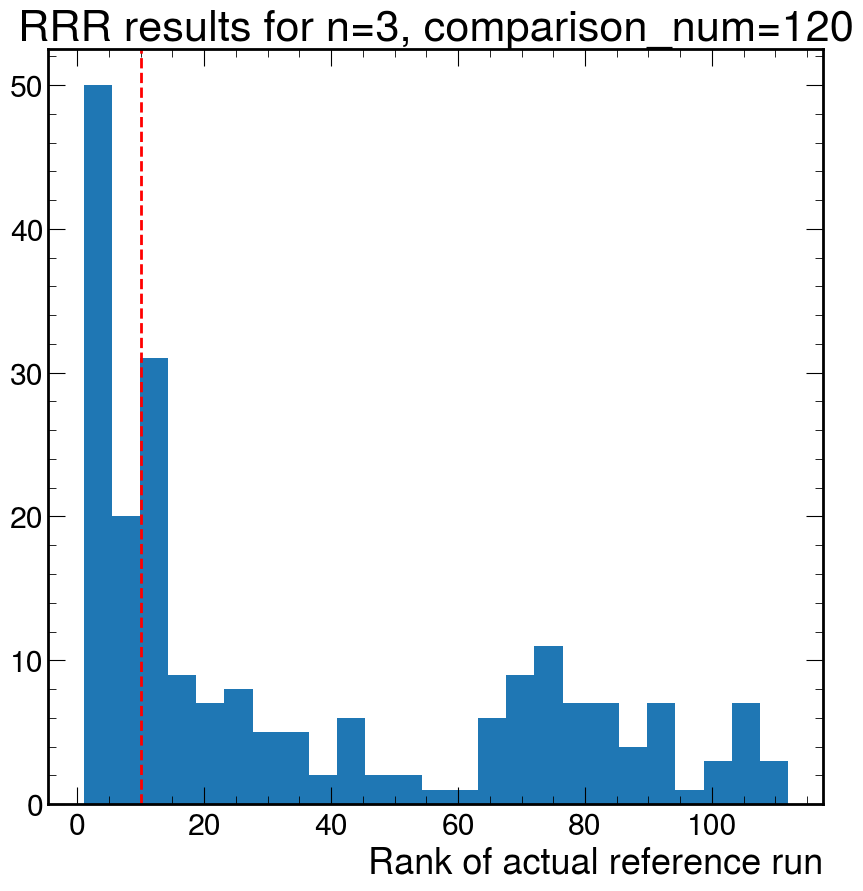
\includegraphics[width=0.5\linewidth]{images/RRR/rrr_testing.png}
    \caption{RRR 2018 rankings for actual reference runs used during certification}
    \label{fig:rrr_hist}
\end{figure}

\begin{figure}[h]
    \centering
    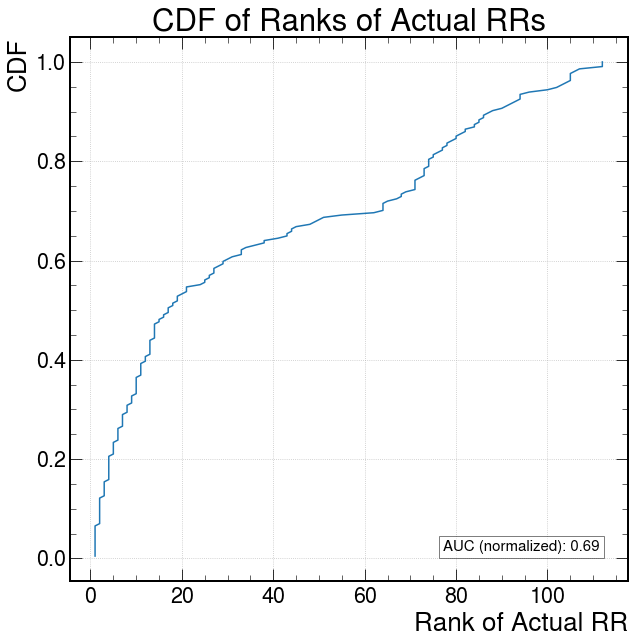
\includegraphics[width=0.5\linewidth]{images/RRR/rrr_test_cdf.png}
    \caption{CDF plot of rankings given to actual reference runs for full 2018 testing}
    \label{fig:rrr_cdf}
\end{figure}

Motivated by these results, further studies and development are being conducted to fine-tune the algorithm. Among these developments is the addition of the previously mentioned standard features (i.e., features that are only standardized and not passed through PCA, leaving them virtually untouched). In addition, the ability to use LS-level features such as, for instance, the mean luminosity or the median HLT physics rate were added to provide more options for the user on what attributes they wanted to prioritize and include in the ranking.

% To validate that the algorithm was acting as expected and to understand its performance in ranking runs, a series of basic statistical tests were run. In these tests, the following primary and PC features were selected.

% \begin{table}[h]
%   \centering
%   \begin{tabular}{|c|c|}
%     \hline
%     Primary features        & PC features                               \\ \hline
%     Energy (TeV)            & HLT physics counter                       \\ 
%     Magnetic field (Tesla)  & Mean recorded luminosity                  \\ 
%     HLT rate                & Mean pileup                               \\ 
%     Run number              & Standard deviation of recorded luminosity \\ 
%     Fill number             & Standard deviation of pileup              \\ 
%                             & Median recorded luminosity                \\ 
%                             & Median pileup                             \\ \hline
%   \end{tabular}
%   \caption{A simple two-column table}
%   \label{tab:ftrs}
% \end{table}

% The target run that was selected was ...